\documentclass[../../sdf/tex/BPSK_system.tex]{subfiles}
\graphicspath{{../../images/}}
%opening
\onlyinsubfile{\title{Homodyne Receiver}}
\date{}

\begin{document}

\onlyinsubfile{\maketitle}

\subsection*{Introduction}

This super-block compresses the function of the following blocks:
\begin{itemize}
\item Local Oscillator;
\item Balanced Beamsplitter;
\item Photodiode;
\item Subtractor;
\item Amplifier;
\item Discretizer;
\item Delayer
\item Bit Decider;
\end{itemize}
\noindent
This compression allows for a cleaner code. 

\subsection*{Input Parameters}

\begin{itemize}
	\item LocalOscillatorOpticalPower
	\item LocalOscillatorOpticalPower\_dBm
	\item LocalOscillatorPhase
	\item TransferMatrix
	\item Responsivity
	\item Amplification
	\item NoiseAmplitude
	\item SamplingRate
	\item Delay
	\item ReferenceValue
\end{itemize}

\subsection*{Functional Description}

The input signal is evaluated and a binary string is generated from this evaluation.
\par
A diagram of the blocks that constitute this super-block, with the corresponding relations is presented in Figure~\ref{fig:physicalsystem}.

\begin{figure}[H]
\centering
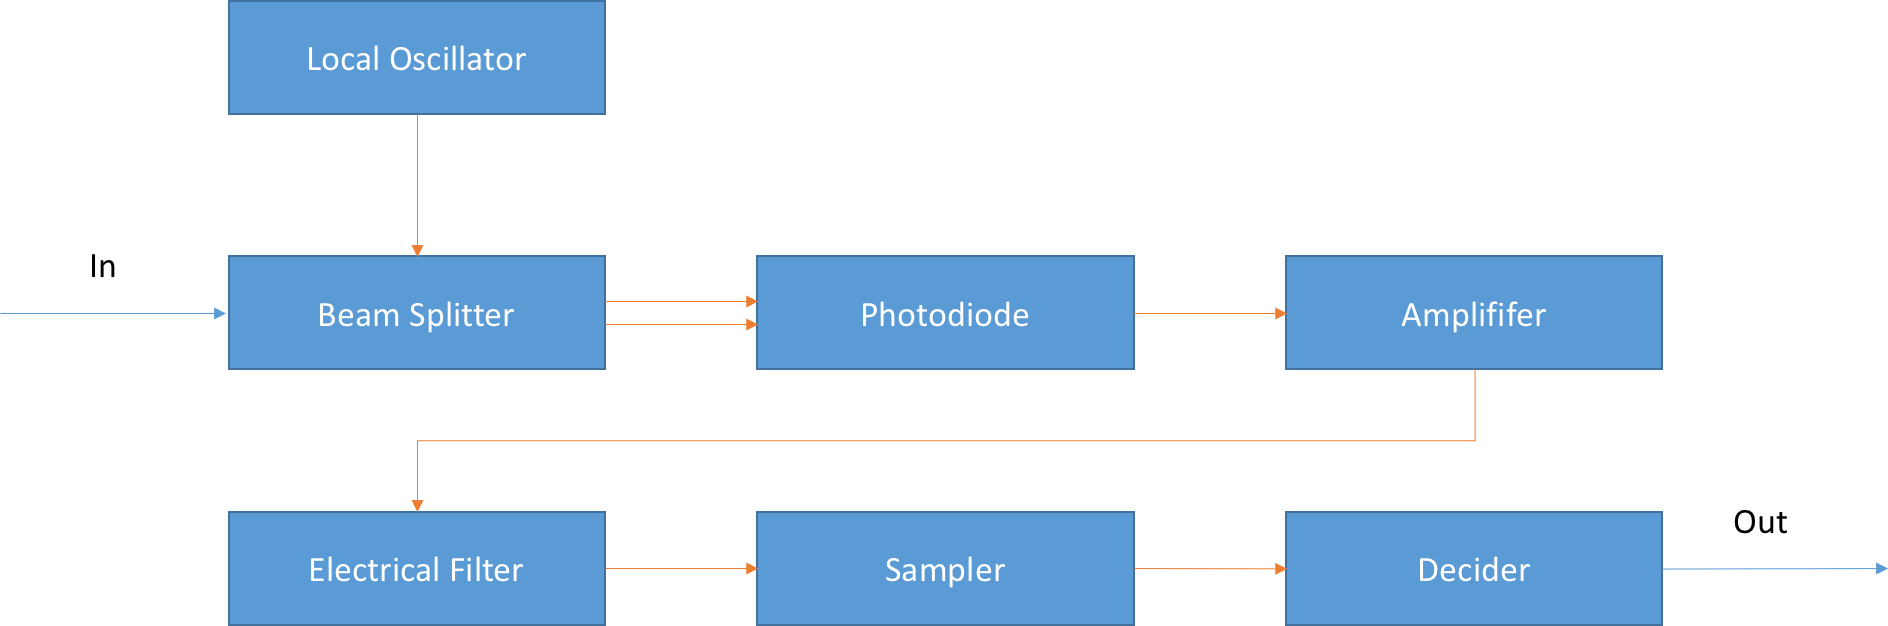
\includegraphics[width=\linewidth]{homodyneblockdiagram.png}
\caption{Homodyne Receiver Block Diagram.}
\label{fig:physicalsystem}
\end{figure}

\subsection*{Inputs}

\textbf{Number}: 1

\textbf{Type}: Sequence of impulses modulated by the filter (OpticalSignal)

\subsection*{Outputs}

\textbf{Number}: 1

\textbf{Type}: Binary String (Binary)

\end{document}